\paragraph{Sơ đồ tuần tự luồng đăng ký tài khoản bằng email}

Luồng nghiệp vụ này mô tả
chi tiết quá trình đăng ký tài khoản mới
sử dụng địa chỉ Email và mật khẩu.

\begin{figure}[H]
\centering
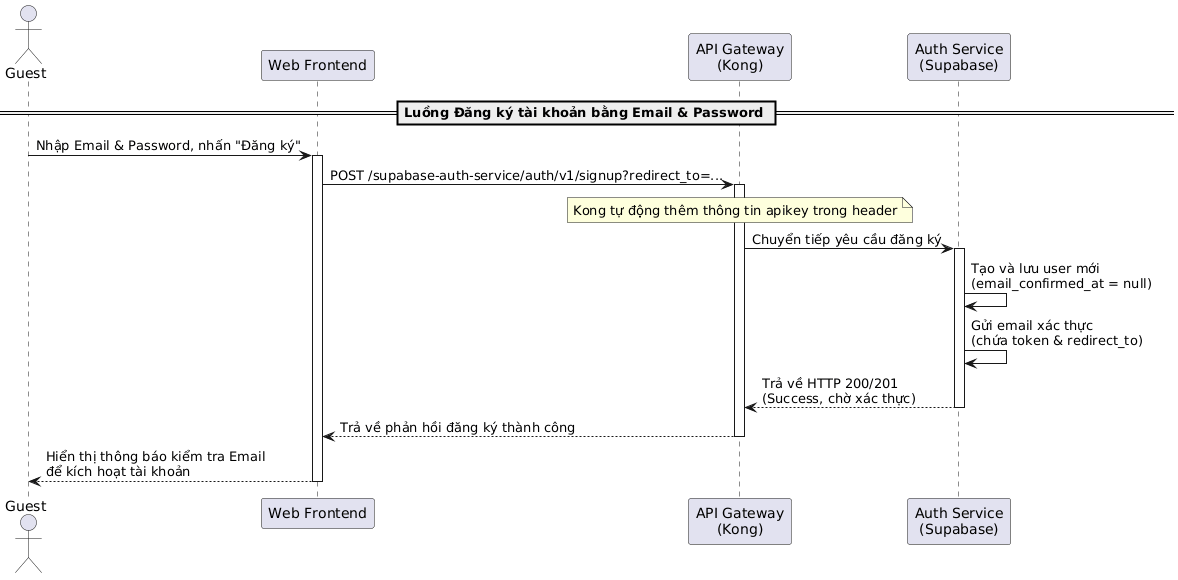
\includegraphics[width=0.95\textwidth]{contents/Sequence/UML-Sequence-GuestEmailPasswordSignup.png}
\caption{Sơ đồ tuần tự luồng đăng ký tài khoản bằng email}
\end{figure}

\begin{table}[H]
\centering
\renewcommand{\arraystretch}{1.3}

\begin{tabular}{|l|l|p{5cm}|}
\hline
\textbf{Thành phần} & \textbf{Phân loại} & \textbf{Vai trò trong hệ thống} \\ \hline
Guest & Actor & Khách vãng lai thực hiện đăng ký tài khoản mới. \\ \hline
Web Frontend & Component & Giao diện web Next.js. \\ \hline
API Gateway (Kong) & Component & Cổng API chuyển tiếp các yêu cầu API. \\ \hline
Auth Service (Supabase) & Microservice & Dịch vụ xác thực xử lý yêu cầu đăng ký, tạo tài khoản mới ở trạng thái chờ kích hoạt và gửi email xác thực. \\ \hline
\end{tabular}
\caption{Các thành phần tham gia luồng đăng ký tài khoản bằng email}
\end{table}

\subparagraph{Mô tả tổng quan}

\begin{itemize}

\item \textbf{Đăng ký tài khoản:}
Khách vãng lai nhập địa chỉ thư điện tử
cùng mật khẩu
và chọn đăng ký trên giao diện.

\item \textbf{Chuyển tiếp đăng ký:}
Giao diện gửi yêu cầu đăng ký
qua cổng API đến Auth Service.

\item \textbf{Tạo tài khoản mới:}
Auth Service tạo tài khoản mới trong CSDL
với trạng thái chưa xác thực thư điện tử.

\item \textbf{Gửi thư xác thực:}
Auth Service gửi thư điện tử xác nhận
chứa mã xác thực
và đường dẫn liên kết kích hoạt đến thư điện tử của người dùng.

\item \textbf{Phản hồi kết quả:}
Auth Service gửi phản hồi đăng ký thành công
và đang chờ xác thực về giao diện.

\item \textbf{Thông báo người dùng:}
Giao diện hiển thị thông báo
đề nghị người dùng kiểm tra hộp thư điện tử để kích hoạt tài khoản.
\end{itemize}
